\documentclass[11pt,letterpaper]{article}
\usepackage[utf8]{inputenc}
\usepackage[left=1in,right=1in,top=1in,bottom=1in]{geometry}
\usepackage{amsfonts,amsmath}
\usepackage{graphicx,float}
% -----------------------------------
\usepackage{hyperref}
\hypersetup{%
  colorlinks=true,
  linkcolor=blue,
  citecolor=blue,
  urlcolor=blue,
  linkbordercolor={0 0 1}
}
% -----------------------------------
\usepackage{fancyhdr}
\newcommand\course{MATH-UA.0252\\Numerical Analysis}
\newcommand\hwnumber{7}                  % <-- homework number
\newcommand\NetIDa{Ryan Sh\`iji\'e D\`u} 
\newcommand\NetIDb{October 28th, 2022}
\pagestyle{fancyplain}
\headheight 35pt
\lhead{\NetIDa\\\NetIDb}
\chead{\textbf{\Large Worksheet \hwnumber}}
\rhead{\course}
\lfoot{}
\cfoot{}
\rfoot{\small\thepage}
\headsep 1.5em
% -----------------------------------
\usepackage{titlesec}
\renewcommand\thesubsection{(\arabic{section}.\alph{subsection})}
\titleformat{\subsection}[runin]
        {\normalfont\bfseries}
        {\thesubsection}% the label and number
        {0.5em}% space between label/number and subsection title
        {}% formatting commands applied just to subsection title
        []% punctuation or other commands following subsection title
% -----------------------------------
\setlength{\parindent}{0.0in}
\setlength{\parskip}{0.1in}
% -----------------------------------
\input{../../command.tex}
\begin{document}

Material taken from \cite[Lecture 6 and 10]{TrefethenBau_97}.

\section{Projectors}
A projector is a square matrix $P$ that satisfies
\begin{align*}
    P^2 = P.
\end{align*}

\subsection{}
Assume $P$ is a projector, show that $I-P$ is also a projector.

\subsection{}
We can show that
\begin{align*}
    & \text{range}(I-P) = \text{null}(P);\\
    & \text{null}(I-P) = \text{range}(P);\\
    & \text{range}(P) \cap \text{null}(P) = 0.
\end{align*}

An orthogonal projector is a projector whose has the subspaces $\text{range}(P)$ and $\text{null}(P)$ orthogonal.

n.b.: An orthogonal projector $P$ is not an orthogonal matrix! Why?

\subsection{}
Show that if $P=P^\top$ symmetric, the projector $P$ is orthogonal (Hint: take one vector in $\text{range}(P)$ and one in $\text{null}(P)$, show that they must be orthogonal to each other). 

The reverse direction holds as well. Therefore the two definition are equivalent.

\subsection{}
A special case of orthogonal projection is projection onto a vector:
\begin{align*}
    P_v = \frac{\ve v \ve v^\top}{\ve v^\top \ve v}.
\end{align*}
Show that it is indeed an orthogonal projector with range $\text{span}(\ve v)$.

\subsection{}
Another orthogonal projection is
\begin{align*}
    P_{\perp v} = I-\frac{\ve v \ve v^\top}{\ve v^\top \ve v}.
\end{align*}
What is its null space? What is its range?

\newpage
\section{Geometric interpretation of Householder reflectors}
\subsection{}
Name $H(\ve v)$ the linear subspace orthogonal to the vector $\ve v$. A reflector across $H(\ve v)$ is 
\begin{align*}
    F_{\ve v} = I - 2 \frac{\ve v \ve v^\top}{\ve v^\top \ve v}.
\end{align*}
Compare this with $P_v$ and $P_{\perp v}$, interpret the formula geometrically.

\begin{figure}[H]
    \centering
    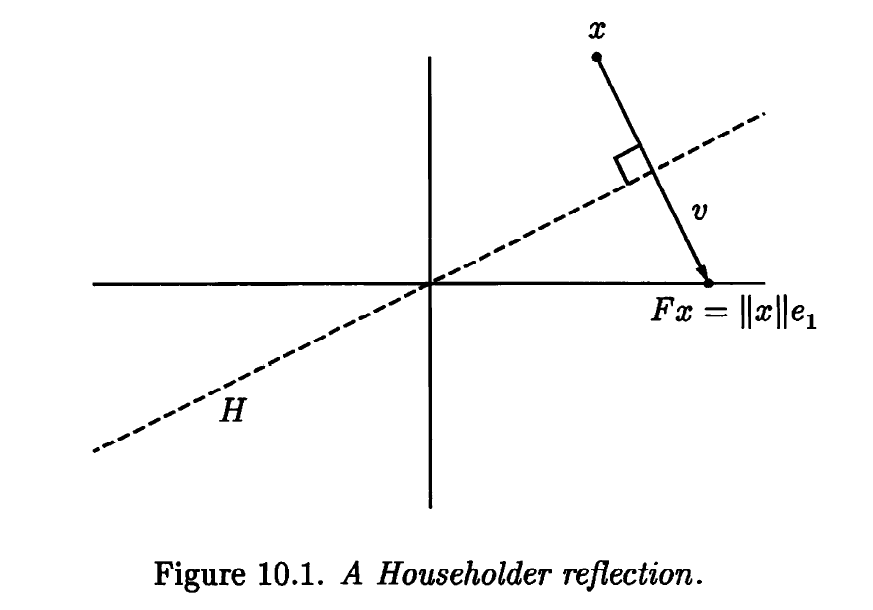
\includegraphics[width = 0.6\textwidth]{figs/TB_HouseholderRef}
\end{figure}

\subsection{}
To use Householder for QR decomposition, we want $F\ve x = c\ve e_1$. We know that $c = \pm\norm{\ve x}_2$. Explain this geometrically.

\subsection{}
From this we have that
\begin{align*}
    \ve v = \ve x- F\ve x =  \ve x \pm \norm{\ve x}\ve e_1.
\end{align*}
From a geometric point of view, why is this the correct formula.





\vfill
\bibliographystyle{alpha}
\bibliography{citation}

\end{document}